%% success_rate.tex — Success rate at different thresholds
%% Data from benchmark run 2026-04-09 (zoom-force, 50 cases)

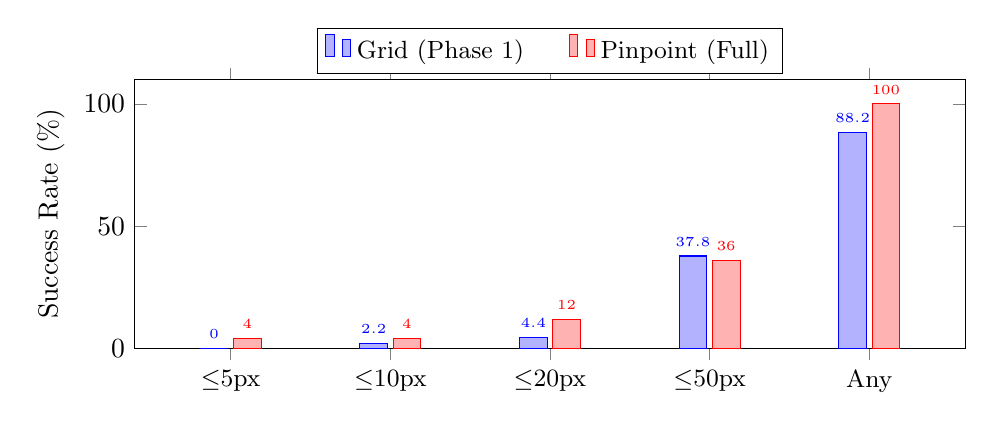
\begin{tikzpicture}
\begin{axis}[
    ybar,
    bar width=10pt,
    width=\columnwidth,
    height=5cm,
    ylabel={Success Rate (\%)},
    symbolic x coords={$\leq$5px, $\leq$10px, $\leq$20px, $\leq$50px, Any},
    xtick=data,
    xticklabel style={font=\small},
    ymin=0, ymax=110,
    legend style={
      at={(0.5,1.02)}, anchor=south,
      legend columns=2, font=\small,
      /tikz/every even column/.append style={column sep=0.5cm}
    },
    nodes near coords,
    nodes near coords style={font=\tiny},
    enlarge x limits=0.15,
  ]

  % Grid: 45/51 success total, threshold rates out of 45 successful
  % <=5: 0/45=0%, <=10: 1/45=2.2%, <=20: 2/45=4.4%, <=50: 17/45=37.8%, any: 45/51=88.2%
  \addplot coordinates {
    ($\leq$5px, 0) ($\leq$10px, 2.2) ($\leq$20px, 4.4) ($\leq$50px, 37.8) (Any, 88.2)
  };

  % Pinpoint: 50/50 success total
  % <=5: 2/50=4%, <=10: 2/50=4%, <=20: 6/50=12%, <=50: 18/50=36%, any: 50/50=100%
  \addplot coordinates {
    ($\leq$5px, 4.0) ($\leq$10px, 4.0) ($\leq$20px, 12.0) ($\leq$50px, 36.0) (Any, 100.0)
  };

  \legend{Grid (Phase~1), Pinpoint (Full)}

\end{axis}
\end{tikzpicture}
